\documentclass[11pt,a4paper]{article}
% \usepackage[margin=1in]{geometry}
\usepackage{amsmath,amssymb}
\usepackage{algorithm}
\usepackage{algorithmic}
\usepackage{tikz}
\usetikzlibrary{positioning}

\title{\vspace{-1cm}
Electronic Supplementary Material\\[4pt]
\large Pseudocode for the Multi--Harmonic Balance Method (MHBM)}
\date{}
\author{}

\begin{document}
\maketitle

% ---------------------------------------------------------
\section*{Algorithm S1: Static Configuration (Summary)}
% \begin{algorithm}[h!]
% \caption{Static configuration (pseudocode)}
\begin{algorithmic}[1]
\STATE \textbf{Input:} cable length $L$, weight $W$, stiffnesses $EA$ and $EI$, node count $N$,
      anchor coordinates $(x_{\text{hang}},z_{\text{hang}})$, and fairlead coordinates $(x_{\text{end}},z_{\text{end}})$.
\STATE Solve a catenary system such that an inextensible cable passes through anchor and fairlead, obtaining parameters $(c_1,c_2,T_0,S_\ell)$.
\STATE Discretize the arc coordinate $S_0\in[0,L]$ and compute approximate static positions $(x_i,z_i)$.
\STATE Estimate static angles $\phi_i^{\text{approx}}$ from finite differences.
\STATE Construct initial guesses for strain and angle fields.
\STATE Solve the finite-difference static equilibrium system to obtain $e_i^0$ and $\phi_i^0$.
\STATE Define static tension $T_i^0 = EA\,e_i^0$.
\end{algorithmic}
% \end{algorithm}
\section*{Algorithm S2: Multi-Harmonic Balance Method (MHBM)}
% \begin{algorithm}[h!]
% \caption{MHBM for periodic fairlead response (pseudocode)}
\begin{algorithmic}[1]

% --- Harmonics ---
\STATE \textbf{Harmonic representation}
\STATE Choose the number of harmonics $N_h$ and represent any periodic quantity $q(t)$ by
\[
q(t) \approx \frac{q_0}{\sqrt{2}} +
\sum_{h=1}^{N_h} \big( q_h^{\cos}\cos(h\omega t) + q_h^{\sin}\sin(h\omega t) \big).
\]
\STATE Set $N_{\text{h,eff}} = 2N_h+1$.

% --- Unknown vector ---
\STATE \textbf{Unknown vector and index map}
\STATE Build the global unknown vector $X$ containing all Fourier coefficients for $u,v,e,\phi$ at all nodes.
\STATE Build an index map linking each coefficient in $X$ to a node and variable.

% --- Initial guess ---
\STATE \textbf{Initial guess $X_0$}
\STATE Use static fairlead angle $\phi_N^0$ to project the imposed fairlead motion into tangential and normal components.
\STATE Initialise harmonic coefficients for fairlead $u,v$ to match imposed motion.
\STATE Initialise strain and angle coefficients from static fields plus small harmonic perturbations.

% --- Residual ---
\STATE \textbf{Residual assembly}
\STATE For each collocation time point:
\begin{itemize}
  \item Reconstruct $u_i(t)$, $v_i(t)$, $e_i(t)$ and $\phi_i(t)$ from $X$.
  \item Compute spatial derivatives and curvature by finite differences.
  \item Evaluate tension and bending forces using $EA$, $EI$, and $(e_i^0,\phi_i^0)$.
  \item Compute fluid-relative velocities and hydrodynamic drag forces.
  \item Enforce the semi-discrete equations of motion and boundary conditions.
\end{itemize}
\STATE Collect all equations into the global residual vector $R(X)$.

% --- Nonlinear solve ---
\STATE \textbf{Nonlinear solve}
\STATE Solve the nonlinear system $R(X)=0$ using Newton or Levenberg--Marquardt to obtain $X_{\text{sol}}$.

% --- Reconstruction ---
\STATE \textbf{Reconstruction and fairlead tension}
\STATE For a dense set of times $t$ over one period, reconstruct $u(t)$, $v(t)$, $e(t)$, $\phi(t)$ at the fairlead.
\STATE Compute total angle $\phi_{\text{tot}}(t)$ and total strain.
\STATE Compute fairlead tension as
\[
T_{\text{fairlead}}(t) = T_{\text{fairlead}}^{0} + EA\,e_{\text{dyn}}(t).
\]

\end{algorithmic}
% \end{algorithm}

% ---------------------------------------------------------
\section*{Flowchart of the MHBM Workflow}
% ---------------------------------------------------------

\begin{center}
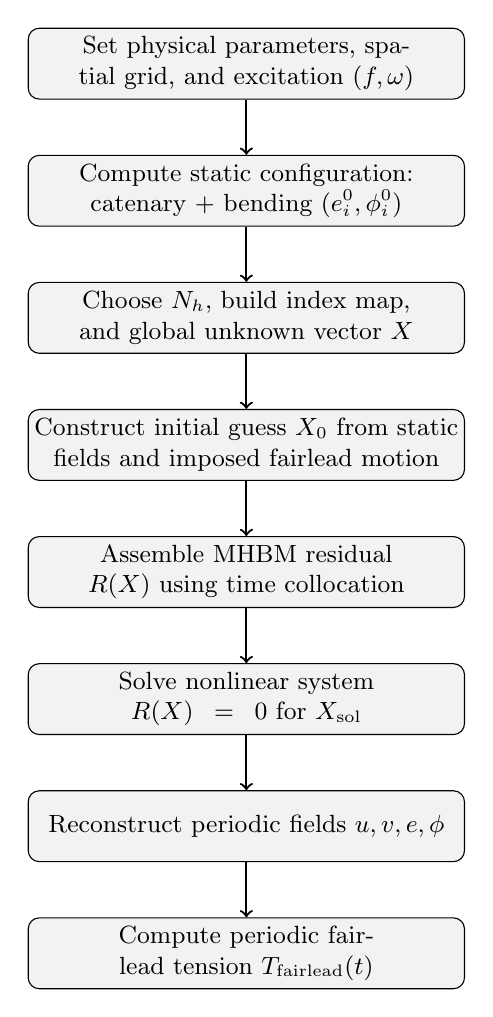
\begin{tikzpicture}[
    node distance=0.7cm,
    every node/.style={font=\small, align=center},
    box/.style={rectangle, draw, rounded corners, fill=gray!10,
                text width=5.4cm, minimum height=0.9cm, inner sep=2pt},
    arrow/.style={->, thick}
]

\node[box] (p1) {Set physical parameters, spatial grid, and excitation $(f,\omega)$};
\node[box, below=of p1] (p2) {Compute static configuration:\\ catenary + bending $(e_i^0,\phi_i^0)$};
\node[box, below=of p2] (p3) {Choose $N_h$, build index map, and global unknown vector $X$};
\node[box, below=of p3] (p4) {Construct initial guess $X_0$ from static fields and imposed fairlead motion};
\node[box, below=of p4] (p5) {Assemble MHBM residual $R(X)$ using time collocation};
\node[box, below=of p5] (p6) {Solve nonlinear system $R(X)=0$ for $X_{\mathrm{sol}}$};
\node[box, below=of p6] (p7) {Reconstruct periodic fields $u,v,e,\phi$};
\node[box, below=of p7] (p8) {Compute periodic fairlead tension $T_{\mathrm{fairlead}}(t)$};

\draw[arrow] (p1) -- (p2);
\draw[arrow] (p2) -- (p3);
\draw[arrow] (p3) -- (p4);
\draw[arrow] (p4) -- (p5);
\draw[arrow] (p5) -- (p6);
\draw[arrow] (p6) -- (p7);
\draw[arrow] (p7) -- (p8);

\end{tikzpicture}
\end{center}

\end{document}
